\documentclass[10pt,a4paper]{article}
\usepackage[utf8]{inputenc}
\usepackage[a4paper, margin=1.8cm, top=2.0cm, bottom=2.0cm]{geometry}
\usepackage{amsmath,amssymb}
\usepackage{xcolor}
\usepackage[most]{tcolorbox}
\usepackage{booktabs}
\usepackage{colortbl}
\usepackage{fancyhdr}
\usepackage{graphicx}
\usepackage{enumitem}

% Exact colors from original Claude summary
\definecolor{themeblue}{rgb}{0.1686, 0.3529, 0.5294}   % #2B5A87
\definecolor{lightbg}{rgb}{0.9098, 0.9333, 0.9569}     % #E8EEF4
\definecolor{accentred}{rgb}{0.7843, 0.2706, 0.2275}   % #C8453A

% Header and Footer
\pagestyle{fancy}
\fancyhf{}
\fancyhead[L]{\textcolor{themeblue}{\small Lecture 1 --- Data exploration}}
\fancyhead[R]{\textcolor{themeblue}{\small Summary Sheet}}
\renewcommand{\headrulewidth}{0.5pt}
\renewcommand{\headrule}{\hbox to\headwidth{\color{themeblue}\leaders\hrule height \headrulewidth\hfill}}
\fancyfoot[C]{\thepage}

\begin{document}

% Title Block
\begin{center}
    {\LARGE\bfseries\color{themeblue} High Dimensionality}\\[3pt]
    {\small\itshape Summary sheet --- Deep Learning (S.-A. Berrani, ENSIA 2026--2027)}\\[3pt]
    \textcolor{themeblue}{\rule{\textwidth}{0.6pt}}
\end{center}

% Core Idea & Notation Box
\begin{tcolorbox}[
    colframe=themeblue,
    colback=lightbg,
    coltitle=white,
    fonttitle=\bfseries\sffamily,
    title={Core idea \& notation},
    arc=2mm,
    boxrule=0.6pt,
    left=8pt, right=8pt, top=5pt, bottom=5pt
]
\textit{High-dimensional} data (dimension $> 3$) escapes our intuition: distances, volumes and sample requirements behave in counter-intuitive ways. All these difficulties are called the \textbf{dimensionality curse}. Analysis, exploration, processing and management all become harder.
\begin{itemize}[leftmargin=14pt, itemsep=2pt, topsep=2pt]
    \item $d$ --- dimension (number of variables); $n$ --- number of individuals (samples).
    \item $V_d(r)$ --- volume of a $d$-dimensional hyper-sphere of radius $r$; $\varepsilon$ --- width of the frame in the hyper-cube.
    \item $D_{\min}, D_{\max}$ --- distance from a query point to its nearest / furthest neighbour.
\end{itemize}
\end{tcolorbox}

\vspace{5pt}

% Section 1
\noindent{\Large\bfseries\color{themeblue} 1. The dimensionality curse}\\[4pt]
\textbf{Optimization:} difficulty of optimizing in high-dimensional spaces with \textit{exhaustive} methods.\\
\textbf{Statistics:} to keep the same reliability of an estimate, the number of samples must grow \textit{exponentially} with $d$.\\[4pt]
\begin{tcolorbox}[
    colframe=accentred,
    colback=white,
    arc=1.5mm,
    boxrule=0.5pt,
    left=8pt, right=8pt, top=5pt, bottom=5pt
]
\textbf{Identification.} More variables \textit{and} more individuals $\Rightarrow$ less intuition, costly processing, harder analysis. Whenever a method needs ``enough points in every region of space'', expect the curse.
\end{tcolorbox}

\vspace{3pt}
\noindent{\large\bfseries\color{themeblue} 1.1 Quantities that grow exponentially with $d$}\\[3pt]
To cover or explore all possible configurations, the required effort grows exponentially with dimension:
\begin{center}
\small
\begin{tabular}{lll}
\toprule
\rowcolor{lightbg}
\textbf{Quantity} & \textbf{Growth} & \textbf{Illustration} \\
\midrule
Binary combinations of $d$ variables & $2^d$ & Each new dimension doubles the number of states ($10 \to 10^3, 20 \to 10^6$) \\
\bottomrule
\end{tabular}
\end{center}

\vspace{5pt}

% Section 2
\noindent{\Large\bfseries\color{themeblue} 2. Loss of the notion of distance}\\[4pt]
When $d$ increases (under data uniformly distributed on all dimensions and independent):
\begin{itemize}[leftmargin=14pt, itemsep=2pt, topsep=2pt]
    \item the distance to the \textbf{nearest} neighbour increases;
    \item the distance to the \textbf{furthest} neighbour increases;
    \item but $D_{\min}$ increases \textbf{faster} than $D_{\max}$.
\end{itemize}
\textbf{Limit:}
\[
d \to \infty \implies \fbox{$D_{\min} \approx D_{\max}$} \qquad \left(\text{i.e. } \frac{D_{\max}}{D_{\min}} \to 1\right)
\]
\begin{tcolorbox}[
    colframe=accentred,
    colback=white,
    arc=1.5mm,
    boxrule=0.5pt,
    left=8pt, right=8pt, top=5pt, bottom=5pt
]
\textbf{\color{accentred}Consequence.} Nearest and furthest neighbours become indistinguishable: all points look equally far apart, so distance-based methods (nearest neighbour, clustering with Euclidean distance) lose meaning.
\end{tcolorbox}

\vspace{6pt}

% Section 3 (Flows naturally onto Page 1)
\noindent{\Large\bfseries\color{themeblue} 3. Volume of the hyper-sphere}\\[4pt]
\noindent
\begin{minipage}[c]{0.52\textwidth}
\textbf{Formula:}
\[
V_d(r) = \frac{\pi^{d/2}}{\Gamma(\frac{d}{2} + 1)} r^d
\]
\textcolor{accentred}{\textbf{Behavior (unit sphere, $r = 1$):}}
\begin{itemize}[leftmargin=12pt, itemsep=2pt, topsep=2pt]
    \item The volume initially increases, reaches its maximum at \textbf{$d = 5$} ($V_5(1) \approx 5.26$), and then rapidly collapses to $0$ as $d \to \infty$.
    \item Relative to the enclosing cube (side 2, volume $2^d$), the sphere's volume ratio drops exponentially to $0$:
    \[
    \lim_{d \to \infty} \frac{V_{\text{sphere}}}{V_{\text{cube}}} = 0
    \]
    \item \textit{The volume of the cube concentrates in its corners}.
\end{itemize}
\end{minipage}\hfill
\begin{minipage}[c]{0.45\textwidth}
\centering
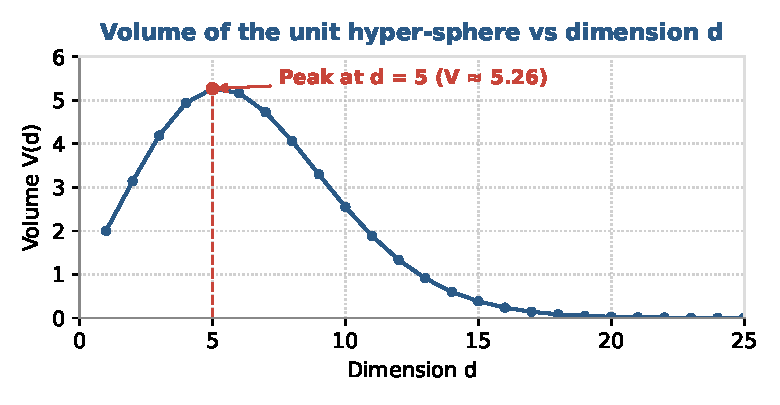
\includegraphics[width=\linewidth]{sphere_volume.pdf}
\end{minipage}

\newpage

% Section 4 (Page 2)
\noindent{\Large\bfseries\color{themeblue} 4. Exercise: hyper-cube and its frame}\\[8pt]
\noindent
\begin{minipage}[c]{0.68\textwidth}
\textbf{Setup:} points uniformly distributed in the hyper-cube $[0, 1]^d$. The \textbf{frame} (grey) is the set of points at distance $\le \varepsilon$ from the edge, $0 < \varepsilon < \frac{1}{2}$. The remaining inner hyper-cube is $[\varepsilon, 1 - \varepsilon]^d$, of side $1 - 2\varepsilon$.\\[8pt]
\textbf{Probabilities (volume ratios):}
\[
P(\text{inner}) = \frac{\text{Vol}([\varepsilon, 1-\varepsilon]^d)}{\text{Vol}([0, 1]^d)} = (1 - 2\varepsilon)^d, \qquad \fbox{$P(\text{frame}) = 1 - (1 - 2\varepsilon)^d$}
\]
\textbf{Asymptotic limit ($d \to \infty$):}
Since $0 < 1 - 2\varepsilon < 1$, $(1 - 2\varepsilon)^d \xrightarrow{d \to \infty} 0$, hence:
\[
\lim_{d \to \infty} P(\text{frame}) = 1
\]
\end{minipage}\hfill
\begin{minipage}[c]{0.28\textwidth}
\centering
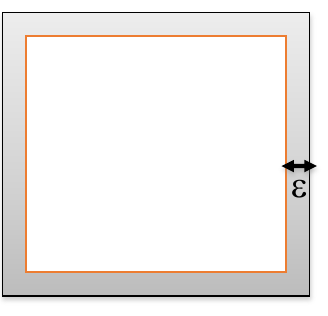
\includegraphics[width=\linewidth]{hypercube_frame.png}\\[4pt]
{\footnotesize\textit{Hyper-cube and $\varepsilon$-frame}}
\end{minipage}

\vspace{10pt}
\noindent\textcolor{accentred}{\textbf{Example:}} $\varepsilon = 0.05$ (so $1 - 2\varepsilon = 0.9$):
\[
d = 2: 0.19, \quad d = 3: 0.27, \quad d = 10: 0.65, \quad d = 50: 0.995, \quad d = 100: 0.99997
\]
Number of dimensions for $P(\text{frame}) \ge p$: $d \ge \frac{\ln(1 - p)}{\ln(1 - 2\varepsilon)}$; for $p = 0.99$: $d \ge 43.7$, i.e. $\mathbf{d \ge 44}$.

\vspace{10pt}
\begin{tcolorbox}[
    colframe=accentred,
    colback=white,
    arc=1.5mm,
    boxrule=0.5pt,
    left=8pt, right=8pt, top=6pt, bottom=6pt
]
\textbf{What we notice.} The probability curve increases and saturates at 1: in high dimension, \textbf{almost every point lies near the edge} (in the $\varepsilon$-frame) and the ``centre'' is empty. Data are sparse and isolated.
\end{tcolorbox}

\vspace{16pt}

% Section 5
\noindent{\Large\bfseries\color{themeblue} 5. Solutions}\\[8pt]
\begin{center}
\small
\begin{tabular}{p{0.18\textwidth}p{0.38\textwidth}p{0.36\textwidth}}
\toprule
\rowcolor{lightbg}
 & \textbf{1. Reduce the variables} & \textbf{2. Reduce the instances} \\
\midrule
\textbf{Idea} & Create new variables from the original ones while losing as little information as possible & Partition the dataset by grouping similar individuals \\
\addlinespace[6pt]
\textbf{Acts on} & Columns (features), $p \to q < p$ & Rows (individuals) \\
\addlinespace[6pt]
\textbf{Example} & \textbf{PCA} (Principal Component Analysis) & \textbf{Clustering} (unsupervised classification) \\
\bottomrule
\end{tabular}
\end{center}

\end{document}
